\chapter{Proposta de solução}
\label{chap:solution_propositon}

No contexto de videogames que utilizam reações visuais/auditivas como mecânica essencial de jogabilidade, existe uma alta sensibilidade à latência de \textit{inputs}. Como forma de mitigar esse problema, a técnica de previsão no lado do cliente, como descrito na \secref{sec:client_side_prediction}, é implementada em diversos \textit{games} e é muito bem vista pelos jogadores \cite{rollback_success}.

Similarmente, ao observar ambientes musicais \textit{online}, percebe-se o mesmo requisito de baixa latência para manter a sensação fluidez e sincronia entre os participantes, como descrito na \secref{sec:problem}. Portanto, questiona-se: é possível aplicar técnicas de predição no lado do cliente nesse contexto, de forma a permitir sessões artísticas satisfatórias entre os músicos?

Evidentemente, apesar de compartilharem um requisito de baixa tolerância a latência, as naturezas dos problemas são significativamente divergentes. A mera implementação de previsão no lado do cliente no contexto musical implica em dois grandes problemas: (1) a impossibilidade de retornar ao último momento da música em caso de erro na previsão e; (2) a enorme dimensionalidade da representação digital de áudio.

A técnica de previsão no lado do cliente, quando aplicada a videogames, baseia-se no fato que os eventuais retornos aos estados anteriores às previsões em caso de erros não são suficientemente prejudiciais à experiência do jogador. No contexto de música, no entanto, devido sua natureza contínua na linha do tempo, o conceito de estados não pode ser replicado e, portanto, não faz sentido retornarmos a um momento anterior.
 
Ademais, a quantidade de \textit{inputs} produzidos pelos jogadores é ínfima quando comparada a representação de áudio digital. Estima-se que os jogadores profissionais mais técnicos de \textit{Super Smash Bros. Melee}, um jogo de luta em plataformas, produzem em média cerca de 6 \textit{inputs} por segundo \cite{melee_inputs_per_second}, variando de acordo com o momento do jogo. Por outro lado, uma transmissão de áudio com \textit{sample rate} de 44,1 Khz produz consistentemente, por definição, 44.100 diferentes valores no mesmo espaço de tempo \cite{jukebox_dimension}. O modelo preditivo proposto por Bernier \cite{client-side-prediction} replica os últimos \textit{inputs} reconhecidos pelo servidor; se aplicássemos o mesmo método no contexto musical, efetivamente estaríamos ``atrasando'' os \textit{inputs} de áudio, portanto, perdendo a sincronia entre os participantes.

Portanto, a acurácia do modelo preditivo em ambientes musicais é de suma importância, uma vez que a ``volta no tempo'' é impossível. Atingir esse alto nível de acurácia, por sua vez, é um enorme desafio, dada a dimensionalidade da representação de áudio digital. Naturalmente, o tempo total gasto na geração da previsão não pode exceder o tempo da janela prevista - caso ocorra, retornaremos ao mesmo problema enfrentado pelas soluções síncronas apresentadas na sessão \secref{sec:delay-based-audio-solutions}.

\section{Adaptação do \textit{client-side prediction} no contexto musical \textit{online}}

Propomos, então, uma variação da implementação de Bernier \cite{client-side-prediction} de previsão no lado do cliente, para sua aplicação no contexto musical (\figref{fig:rollback_music_diagram}). Similarmente à técnica original, janelas de áudios são previstos baseando-se em entradas anteriores. Entretanto, nenhuma correção é realizada em casos de erro, mantendo a linearidade da música.

\begin{figure}[htbp]
\centering
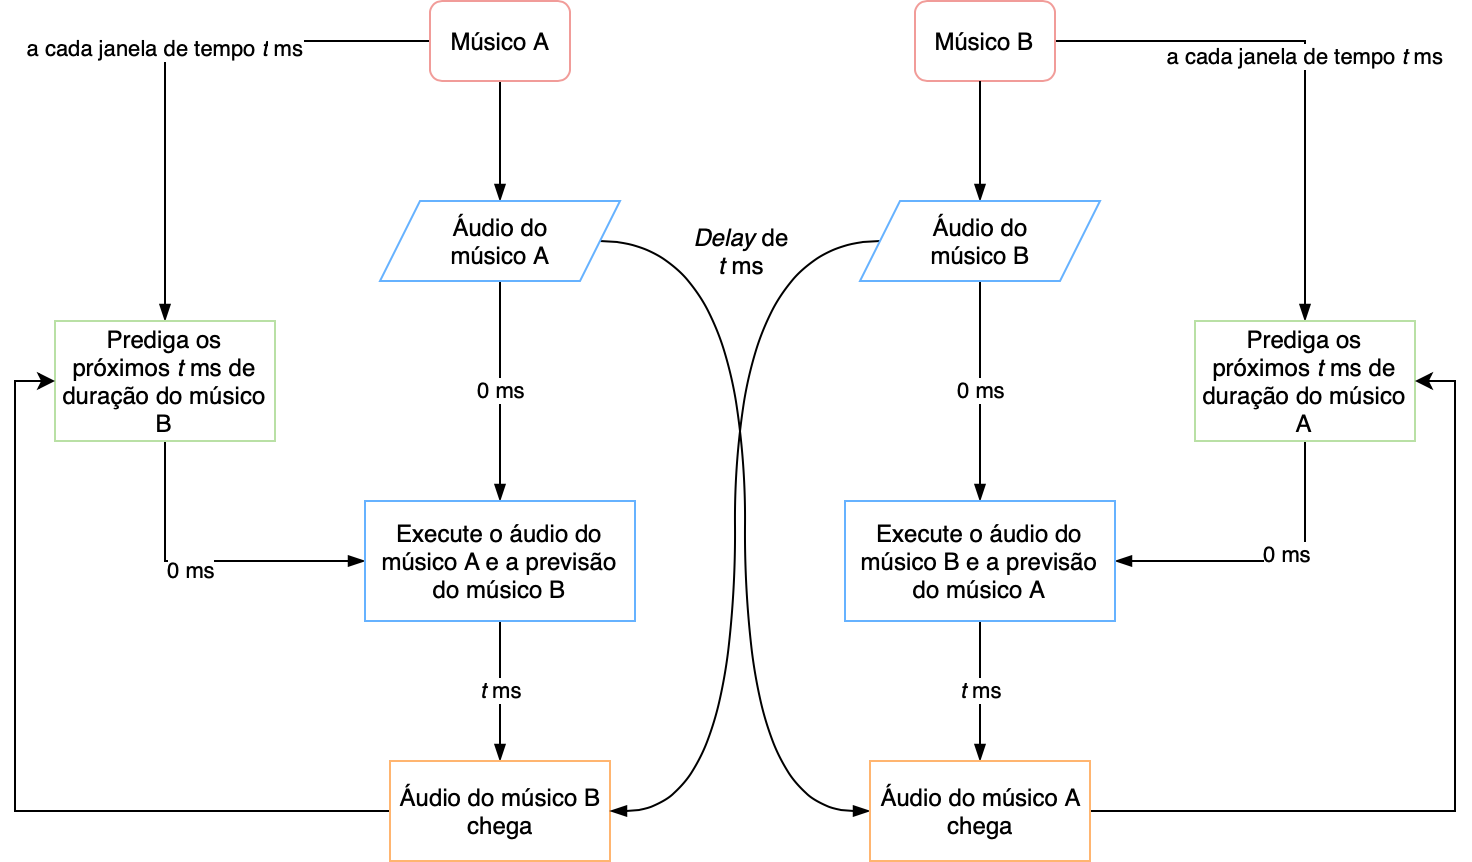
\includegraphics[width=1\textwidth]{images/rollback-music.png}
\caption{Diagrama demonstrando a adaptação do algoritmo de previsão no lado do cliente aplicado para \textit{streaming} colaborativo de música \textit{online}. Na imagem, $t$ representa a duração da janela de previsão, medido em milissegundos.}
\label{fig:rollback_music_diagram}
\end{figure}

Em Bernier, a janela de tempo de cada conjunto de previsões é definida de acordo com o FPS e a velocidade de conexão entre os participantes. Para adaptação musical, além do tempo de ida e volta dos pacotes entre os participantes (denominado \textit{ping}), propomos a utilização de outros parâmetros para a decisão dessa janela, como o BPM (batimentos por minuto) da música tocada junto à informação dos compassos musicais e também, por simplicidade, valores múltiplos de 1 segundo. A escolha dessa janela é fundamental - durações muito longas possuem muita informação, porém, são mais difíceis de processar e mais suposições terão que ser realizadas na previsão; e o inverso ocorre para janelas muito curtas.

Propomos, portanto, dois modelos preditivos para música, explorados em dois ciclos de pesquisa. No \chapref{chap:lstm}, o primeiro ciclo, utilizamos a arquitetura de aprendizagem de máquina em camadas LSTM (\textit{Long short-term memory)} \cite{lstm} para gerar sequências de sinais digitais, baseadas nas entradas anteriores. Já no \chapref{chap:dtw}, no segundo ciclo, usamos o algoritmo DTW (\textit{Dynamic Time Warping}) \cite{dtw} para identificar janelas semelhantes em uma base de dados e, a partir dessa informação, reproduzir a próxima janela de áudio, também armazenada na mesma base de dados.

É válido mencionar que, no entanto, pela natureza imprevisível das improvisações musicais, esse caso de uso não deve ser bem aplicado em nossa solução proposta. Porém, para bases e sequências de acordes, onde é mais fácil prever as próximas entradas, o uso de nossa solução é melhor adequado.

...

\section{Métricas de sucesso dos modelos preditivos}
\label{sec:success_metrics}

Como mencionado, existem alguns requisitos que os modelos preditivos propostos precisam cumprir para serem considerados bem sucedidos. Em cada ciclo, diferentes metodologias foram utilizadas para demonstrar essas métricas.

\subsection{Corretude das previsões}
\label{subsec:prediction_correctness}

Devido à característica de linearidade de tempo que a música possui, não é possível ``retornar'' a um estado passado da música. Dessa forma, é importante que os modelos sejam os mais acurados possíveis.

Dada a natureza da predição, não é esperado que as sequências geradas sejam integralmente fidedignas às sequências reais. No entanto, isso não é um requisito para produzir resultados positivos, sendo realmente importante que os áudios previstos tenham a mesma ``intenção'' que a reprodução original.

Dessa forma, o critério de sucesso dessa métrica é, para as sequências previstas, que seja imperceptível, em tempo real, que haja diferenças entre as sequências originais; de forma que um músico, ao ouvir ambas as sequências, reagiria musicalmente da mesma maneira ou de maneira similar.

Note que, por se tratar de um critério abstrato, quantificar essa métrica pode não representar bem o seu sucesso. Em cada um dos ciclos, utilizamos diferentes metodologias (demonstrados em \secref{sec:lstm_metodology} e \secref{sec:dtw_metodology}) para medi-la, visando sempre satisfazer o critério estabelecido.

\subsection{Tempo de geração de previsões}
\label{subsec:time_metric}

Supondo que \textit{t} é o tempo escolhido das janelas de previsão de áudio e \textit{p} é o tempo levado para gerar essas previsões, é imprescindível para o sucesso dos modelos preditivos que $t \leq p $. Caso contrário, o tempo excedente de processamento cria um \textit{delay} entre o que está sendo executado pelo músico remoto e o que está sendo reproduzido localmente e, consequentemente, causando dessincronia entre os músicos.

Ao contrário do critério de corretude na \secref{subsec:prediction_correctness}, essa métrica consegue ser medida precisamente. Será considerado bem sucedida o modelo preditivo que produzir sequências em um tempo menor que a duração do áudio gerado.

\section{Coleta de dados e simulação do ambiente musical \textit{online}}
\label{sec:data_gathering}

Para realizar os experimentos, procuramos simular, de forma simples, um ambiente colaborativo musical \textit{online} \textit{peer-to-peer}, do ponto de vista do músico local. Nosso conjunto de dados, dessa forma, contém pares de arquivos de música com as seguintes regras:

\begin{enumerate}
    \item Ambos arquivos reproduzem a mesma sequência de uma música, porém, em performances diferentes;
    \item Ambos arquivos consistem de apenas um instrumento;
    \item Ambos arquivos consistem do mesmo instrumento.
\end{enumerate}

A Regra 1 visa simular diferentes reproduções de uma a mesma sessão de uma música, porém, de formas diferentes, similarmente a como ser humano o faria. A Regra 2, apesar de não obrigatória em transmissões em casos reais, simplifica o processamento e geração de previsão dos áudios; além disso, não é esperado que vários músicos compartilhem do mesmo canal de transmissão. Por último, a Regra 3 complementa a as duas regras anteriores, garantindo a mesma sequência de áudio performada de diferentes maneiras pelo mesmo instrumento.

Para cada par, podemos nomear o primeiro arquivo $A$ e o segundo $B$, onde $A$ é classificado como o conjunto de treinamento o $B$ o conjunto de teste. Dessa forma, conseguimos simular um ambiente onde um dos músicos possui o conjunto $A$ treinado em sua máquina e está recebendo o conjunto $B$ do músico remoto.

Para coletar arquivos com esses requisitos, a seguinte abordagem foi realizada, ilustrada na \figref{fig:data_gathering}: (1) buscou-se músicas onde a mesma sequência de acordes e notas era reproduzida em diferentes sessões (por exemplo, uma introdução que serve de motivo para a música); (2) depois, isolou-se apenas um instrumento; (3) identificou-se as sessões repetidas e, por último; (4) separou-se as sessões isoladamente e criou-se os dois arquivos, um para treinamento e outro para simulação do áudio trasmitido remotamente.

\begin{figure}[htbp]
\centering
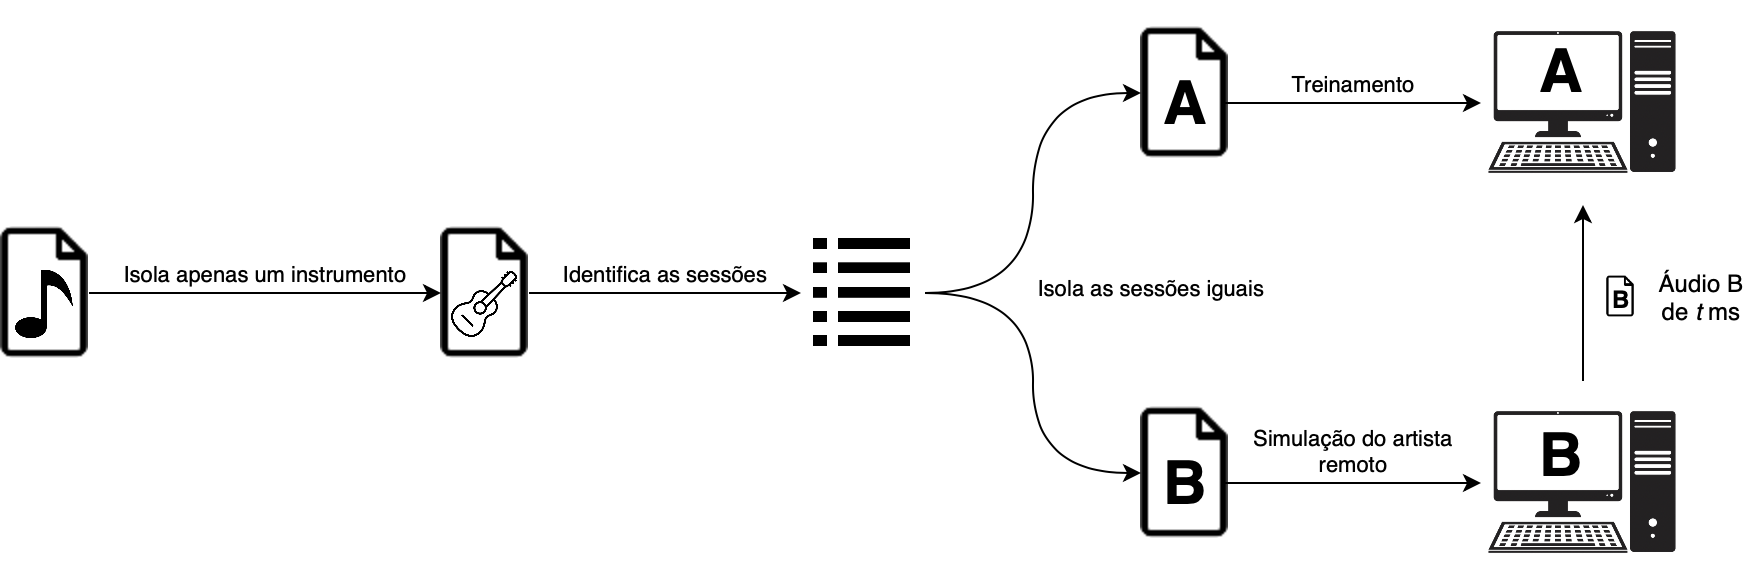
\includegraphics[width=1\textwidth]{images/data-gathering.png}
\caption{Processo de coleta de dados e simulação de um ambiente musical colaborativo \textit{peer-to-peer}. Os arquivos $A$ e $B$ representam uma mesma sessão da música, porém, em performances diferentes.}
\label{fig:data_gathering}
\end{figure}

Essa metodologia de separação de arquivos implica em dizer que a adaptação proposta não pode utilizar nenhum dado futuro do arquivo $B$, pois, no ambiente real, essa informação também não estaria presente. O arquivo $A$, por sua vez, pode ser analisado integralmente. Inclusive, tal análise pode ser realizada em momento anterior às previsões, já que o único tempo relevante a ser metrificado é o que foi levado para gerá-las. Em um ambiente real, o treinamento pode ser realizado antes que os músicos toquem juntos.

As músicas utilizadas nos experimentos foram \textit{Hotel California} (\textit{Eagles}, 1976) - tendo a trilha do violão acústico isolada - e \textit{Message In A Bottle} (\textit{The Police}, 1979) - onde a trilha da guitarra elétrica de base foi isolada.

Os arquivos coletados estão formatados com a extensão WAV, por sua simplicidade, além de suportar o armazenamento de dados não comprimidos, nos fornecendo o máximo de informações possível das trilhas de áudio. O \textit{sample rate} dos arquivo foi de 44,1 KHz com \textit{bit depth} de 16 bits, a mesma qualidade que a escolhida pela mídia dos CD's \cite{cd_quality}.

Os experimentos para cada modelo, demonstrados nos \chapref{chap:lstm} e \chapref{chap:dtw}, foram escritos e executados utilizando a versão gratuita do \textit{Google Colab}, uma aplicação que permite rodar \textit{Jupyter Notebooks} em computadores remotos. Suas especificações são, para CPU, o \textit{Intel(R) Xeon(R) @ 2.20GHz} e, para memória, \textit{Nvidia Tesla K80} \cite{colab_specs}.
\section{Modelos preditivos}

Dada a solução proposta, este trabalho propõe o estudo da viabilidade de dois modelos preditivos - previsão através de (1) geração de novas sequências e (2) indexação e identificação de sequências anteriores. Ambas baseiam-se em extrair informações a partir de entradas anteriores de áudio e apontar um \textit{output} sobre o que classificam ser o mais próximo do dado real futuro - no entanto, possuem diferenças sobre a forma que atingem esse objetivo.

\subsection{Geração de novas sequências}
\label{subsec:new_sequence_generator}

Gerar novas sequências baseando-se em entradas anteriores encaixa-se intuitivamente no conceito de ``previsão'', como descrito no algoritmo de \textit{client-side prediction}. Evidentemente, seu uso em uma adaptação para ambientes musicais foi explorado.

Em nossa adaptação do \textit{client-side prediction}, anteriormente à sessão entre os músicos, um modelo de aprendizagem de máquina é treinado utilizando áudios já conhecidos -  semelhantes, mas não iguais aos que serão produzidos pelo músico remoto. Este modelo receberá como entrada sequências de áudio de $t$ ms de duração e produzirá saídas de mesma duração, como descrito na \figref{fig:generative_model}.

\begin{figure}[htbp]
    \centering
    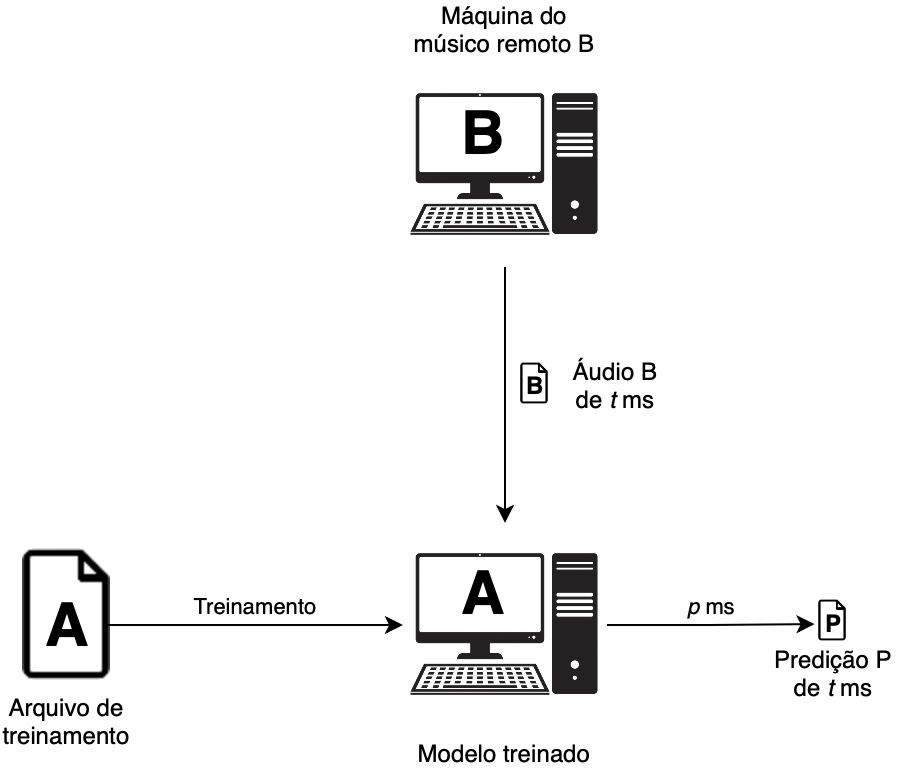
\includegraphics[width=0.75\textwidth]{images/prediction-model.png}
    \caption{Processo de geração de novas sequências através de modelos treinados.}
    \label{fig:generative_model}
\end{figure}

Uma das possibilidades para prever sequências musicais pode ser encontrado no campo de continuação de músicas baseados em um estilo. Dhariwal et. al propõem o \textit{Jukebox}, da \textit{OpenAI}, que usa redes neurais para aprender diferentes gêneros e produzir continuações para músicas \cite{jukebox}. Para o uso em previsões, poderíamos treinar modelos com a música a ser tocada e, para cada pequena sequência, gerar uma continuação. Entretanto, os autores deixam claro que uma das limitações de seu uso é o tempo de renderização - cerca de 8 horas para cada um minuto de áudio gerado \cite{jukebox}. Como o tempo de geração das previsões é bastante sensível em nossa adaptação, essa abordagem foi descartada.

O campo da Aprendizagem de Máquina que visa gerar novas sequências baseando-se nas anteriores é a de Previsão de Séries Temporais (\textit{Time Series Forecasting}). Essa abordagem procura aplicar técnicas para prever continuações de conjunto de dados onde o tempo é uma de suas dimensões \cite{time_series_forecasting}. Podemos classificar, portanto, que previsões de sequências musicais é um subconjunto dos problemas desse campo e, dessa forma, adaptá-la para uso em nossa solução proposta.

Uma das abordagens utilizadas para resolver problemas do conjunto \textit{Time Series Forecasting} é a aplicação das redes neurais recorrentes LSTM (\textit{Long Short-Term Memory}) \cite{lstm}. Tais redes são capazes de aprender conexões de longo prazo. Dessa maneira, elas possuem um memorável poder de predição, funcionando bem em diversos problemas, sendo amplamente usadas atualmente.

A biblioteca \textit{Keras} \cite{keras}, escrita na linguagem de programação Python, implementa modelos de aprendizagem LSTM. Dessa forma, seu uso é bastante promissor para nossa adaptação musical de \textit{Client-Side Prediction}. Exploramos-o no primeiro ciclo de estudos, descrito no \chapref{chap:lstm}.

\subsection{Indexação e identificação de sequências anteriores}
\label{subsec:indexation_and_identification}

No primeiro ciclo de estudos, uma das possibilidades estudadas foi, ao invés de treinar um grande modelo, utilizar cada janela de previsão e treinar pequenos modelos. Para isso, no momento da previsão, precisaríamos de alguma forma de identificar qual modelo melhor se encaixa na sequência de entrada. Com isso, pesquisamos métodos para realizar a identificação das sequências de um banco de dados e, com isso, surgiu a ideia de, ao invés de gerar novas sequências, apenas entregar a que veio após a identificada. 

Para previsão de sequências, a geração de novos valores não é um requisito. Se possuirmos um conjunto de dados, reunindo diferentes sequências e informações sobre quais vieram após tais sequências, poderíamos apenas reproduzi-las. Dessa forma, sugerimos um modelo preditivo que, ao invés de fornecer sequências de áudio inéditas, identifica sequências similares e reproduz a que veio em seguida, como ilustrado na \figref{fig:indexative_model}.

\begin{figure}[htbp]
    \centering
    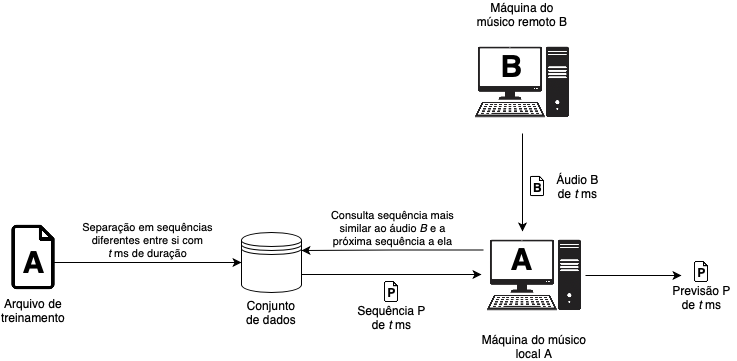
\includegraphics[width=1\textwidth]{images/index-model.png}
    \caption{Processo de identificação de sequência $P$ semelhante à entrada $B$ e entrega da previsão baseada na que veio após a sequência $P$ identificada.}
    \label{fig:indexative_model}
\end{figure}

Além do conjunto de regras apresentados na \secref{sec:data_gathering}, o conjunto de dados de referência que será consultado nesse modelo possui as seguintes regras:

\begin{enumerate}
    \item Todos os arquivos necessitam representar diferentes sessões da música entre si;
    \item Todos os arquivos necessitam possuir duração maior ou igual à $t$ ms, onde $t$ é a duração do arquivo utilizado para consulta de similaridade;
    \item Todos os arquivos requerem que exista um, e apenas um, arquivo que represente a sequência tocada após ele mesmo.
\end{enumerate}

A Regra 1 garante que, ao realizar uma \textit{query} de similaridade entre a sequência de entrada e as armazenadas, haverá no máximo uma correspondência. Tal requisito é importante, pois, se houver mais de uma, haverá mais de uma previsão, causando ambiguidade. A Regra 2 garante que as previsões entregues possuirão pelo menos a mesma duração que as sequências de entrada. Caso sejam menores, a diferença entre as durações causará um atraso de entrega, causando o problema descrito na \subsecref{subsec:time_metric}. Finalmente, a Regra 3 garante que todos os arquivos necessitam possuir outro que represente o que foi tocado após ele, que será de fato entregue como previsão, evitando ambiguidades.

Portanto, tal modelo requer duas técnicas: (1) uma para indexar as sequências de música, respeitando as regras descritas e (2) uma para identificar similaridade entre a sequência de entrada (transmitidas pelo músico remoto) e as sequências armazenadas.

Neste trabalho, realizamos a primeira técnica manualmente. O processo é demonstrado no \chapref{chap:dtw}.

Para a segunda técnica, estudamos alguns que métodos podem ser utilizados para identificação de sequências. A biblioteca Librosa \cite{librosa}, também escrita em Python, implementa algumas ferramentas que podem auxiliar em tal tarefa, como o cálculo da centroide espectral \cite{centroid} de sequências de áudio. O cálculo encontra uma média central entre as frequências presentes em cada janela de tempo da sequência de entrada. Para identificação, poderíamos calcular as centroides de cada sequência no conjunto de dados e comparar com a sequência transmitida pelo músico remoto. Entretanto, apenas a informação das frequências principais não é suficiente para identificar semelhança, uma vez que tal informação não varia tanto para cada janela, principalmente para aquelas que reproduzem o mesmo acorde ou nota.

Entretanto, a mesma biblioteca implementa o algoritmo DTW (\textit{Dynamic Time Warping}) \cite{dtw}, um algoritmo utilizado para comparar e alinhar duas séries temporais. Em nossa adaptação de \textit{client-side prediction}, podemos aplicar DTW nas sequências transmitidas contra o banco de dados. Caso haja uma janela semelhante, o algoritmo a entregará como \textit{output} o \textit{timestamp} do início e fim da identificação.

Dessa forma, o \chapref{chap:dtw} também demonstra como utilizamos o DTW em nossas experimentações, além de sua taxa de sucesso na identificação de janelas semelhantes. Caso essa taxa seja alta o suficiente e a indexação das previsões seja acurada, será possível reproduzir um áudio bastante similar ao transmitido pelo músico remoto.

\subsection{Comparações entre os modelos}

Apesar de ambos os modelos basearem-se em sequências anteriores para gerar ou apontar previsões musicais, as duas abordagens diferem na forma que funcionam. As diferenças implicam em alguns pontos que uma abordagem pode realizar melhor que a outra, assim como o inverso pode ocorrer, descritos na \tabref{tab:models_comparission}.

Por entregar sequências inéditas, o modelo preditivo gerador de novas sequências, descrito na \subsecref{subsec:new_sequence_generator}, é mais flexível que o modelo indexador, descrito na \subsecref{subsec:indexation_and_identification}. Afinal, entradas nunca vistas anteriormente sempre terão previsões geradas, mesmo que não sejam precisas com a realidade. Se aplicarmos sequências não vistas no modelo indexador, nenhuma janela será identificada e, portanto, nenhuma previsão será realizada.

Além disso, para identificar uma janela precisamente, o modelo indexador requisita de mais informações que o modelo gerador, aumentando, portanto, o tempo da janela de previsão. Quanto maior a janela prevista, menor a probabilidade de replicar, de forma similar, a sequência de entrada. 

Por outro lado, pela natureza complexa da representação de áudio, gerar uma sequência de alta qualidade, ainda que precisa, é um grande desafio para o modelo gerador. Por entregar sequências já armazenadas em alta qualidade, o modelo indexador sempre entregará sequências limpas ao ouvido humano, evitando desconfortos dos músicos.

Ademais, a utilização de LSTM, devido à complexidade das redes neurais, pode requerer grandes tempos de processamento \cite{lstm_slow} para gerar as previsões. A busca com DTW, apesar de ser um algoritmo de complexidade $O(N^2)$, pode ser otimizado para grandes bases de dados \cite{dtw_complexity}. Como o tempo de previsão é sensível em nossa adaptação do \textit{client-side prediction} para música, é essencial que o modelo preditivo seja eficiente.

\begin{table}[ht!]
    \centering
    \begin{tabular}{|c|c|c|c|c|}
        \cline{2-5}
        
        \multicolumn{1}{c|}{} & \rotatebox[origin=c]{90}{\makecell{Flexível a \\ novas entradas}} &
        \rotatebox[origin=c]{90}{\makecell{Requer pouca \\ informação}} & \rotatebox[origin=c]{90}{\makecell{Predição de \\ alta resolução}} &
        \rotatebox[origin=c]{90}{\makecell{Rápido \\ processamento}} \\
        
        \hline
        
        Modelo gerador & X & X & & \\ 
        \hline
        
        Modelo indexador & & & X & X \\ 
        \hline
    \end{tabular}
    \caption{Matriz morfológica comparando os dois modelos propostos para adaptação do \textit{client-side prediction} para música.}
    \label{tab:models_comparission}
\end{table}
